\documentclass[a4paper]{article}
\usepackage[utf8]{inputenc}
\usepackage{amsfonts}
\usepackage{amsmath}
\usepackage{amsthm}
\usepackage{graphicx}
\usepackage{array}
\usepackage[footnotesize,bf]{caption}
\usepackage{mathtools}
\usepackage{booktabs}
\usepackage[format=hang]{caption}
\usepackage{subfigure}
\usepackage{textcomp} % For the cent symbol
%\usepackage[font=footnotesize]{subcaption}
\usepackage{varioref}
\captionsetup{justification=justified, singlelinecheck=true}
\usepackage[backend=biber,url=false,doi=false,style=authoryear]{biblatex}
\addbibresource{D:/Rob/Dropbox/PhD/Writing/bibtex/Zotero - IO Modelling.bib}
\addbibresource{D:/Rob/Dropbox/PhD/Writing/bibtex/Zotero - Trade.bib}
\addbibresource{D:/Rob/Dropbox/PhD/Writing/bibtex/Zotero - Networks.bib}
%\addbibresource{/home/rob/Dropbox/PhD/Writing/bibtex/Zotero - IO Modelling.bib}
%\addbibresource{/home/rob/Dropbox/PhD/Writing/bibtex/Zotero - Trade.bib}
%\addbibresource{/home/rob/Dropbox/PhD/Writing/bibtex/Zotero - Networks.bib}
\usepackage{authblk}
\usepackage{attrib}
%\bibliographystyle{elsarticle-harv}
%\nocite{*}
% % Diagramming
\usepackage{tikz}
\usetikzlibrary{arrows,positioning,decorations}
% %

\title{A global inter-country economic model based on linked input-output models \\ DRAFT}
\author[*]{Robert G. Levy}
\author[**]{Thomas P. Ol\'{e}ron Evans}
\author[*]{Alan G. Wilson}

\affil[*]{Centre for Advanced Spatial Analysis, UCL Bartlett Faculty of the Built Environment,
90 Tottenham Court Road, London W1T 4TJ, UK}
\affil[**]{Department of Mathematics, University College London, Gower Street, London WC1E 6BT, UK}


\begin{document}
\maketitle

\begin{abstract}
A global model is presented that can be used as the basis for assessing the impacts of future changes in trade, migration, security and development aid.
The model is based on input-output models for 40 countries, linked with trade data at the sector level.
This is made possible by the World Input-Output Database, a collection of input-output tables for 40 countries across 15 years, and by databases of commodities and services trade from the UN.
The model is constructed using a minimum number of assumptions, and is based as far as possible on empirical observation.
Some initial analysis of the model and its properties are also presented
\end{abstract}

\section{Introduction}
The objective of this paper is to present global economic model that can be used as the basis for assessing the impacts of future changes in trade, migration, security and development aid.
The model presented here represents a first `proof of concept' step towards this ambitious goal.
The economies of individual countries are represented as 35-sector input-output models each of which is linked through trade flows representing imports and exports.
This has recently been made feasible by the publication of the World Input-Output Database (WIOD) \parencite{Timmer2012}, a collection of input-output tables (IOTs) for 40 countries across 15 years, from 1995 to 2009.
The IOTs are linked through data from the UN covering trade in both goods\footnote{comtrade.un.org/db} and services\footnote{unstats.un.org/unsd/servicetrade/}.

The remainder of this paper is structured as follows: 
Section \ref{sec:litreview} gives an overview of existing work in this area.
Section \ref{sec:system} gives a description of the present system and outlines how data is used to calibrate the parameters of the model.
The algorithm used to calculate the output of the model is described in section \ref{sec:algorithm} and some preliminary results are given in section \ref{sec:results}.

Some concluding comments are added in section \ref{sec:conclusions}.

\section{Existing Global Economic Models} \label{sec:litreview}
In the mid-1970s, the creator of input-output economics, Wassily Leontief, had just won the Nobel prize for Economics and took the prestige that this bestowed on him as an opportunity to announce a very ambitious project to model the global economy:

\begin{quotation}
Major efforts are underway to construct a data base for a systematic input-output study not of a single national economy but of the world economy viewed as a system composed of many interrelated parts [...]
Preliminary plans provide for a description of the world economy in terms of twenty-eight groups of countries, with about forty-five productive sectors for each group. \attrib{\cite{Leontief1974}}
\end{quotation}

Some 20 years later, Faye Duchin, a former research assistant of Leontief, described how Leontief's efforts in this area have largely been ignored by economists, describing the departures from the standard, neoclassical modelling in terms of price elasticity and elasticity of substitution as being ``too great to ignore'' \parencite{Duchin2004}. 
See section \ref{sec:iots} for more on this subject.

In the years since Leontief published his global model, Input-output analysis has been largely restricted to regional studies, of which \textcite{Akita1993}, \textcite{Khan1999} and \textcite{Luo2013a} are examples; and studies related to energy and the environment, such as  \textcite{Leontief1970}, \textcite{Joshi1999}, \textcite{Bergh2002} and \textcite{Hendrickson2006}.

However, much more recently, attention has returned to input-output modelling in a global context more generally. \textcite{Tukker2013} describe how several multi-regional input-output (MRIO) models have been developed in the very recent literature.
These are, along with the WIOD which is used in the present model, EORA \parencite{Lenzen2012}, EXIOPOL \parencite{Tukker2013a} and the slightly more mature, and proprietorial GTAP \parencite{Walmsley2012}.

\section{The System Description} \label{sec:system}
The present model has $c$ countries, the economies of which are divided into $s$ productive sectors.
We assume that each sector produces a single good, thus `sector' and `product' are used interchangeably.
All goods are measured in terms of their value, measured in US\$.
For the remainder of this paper the terms `quantity' and `value' will be used interchangeably.
Goods produced domestically are labelled with a dagger superscript ($\dagger$) and imported goods with an asterisk superscript.
Table \ref{tbl:cvars} shows the quantities, taken from data published by the WIOD, which characterise a country's economy for a particular year.
Note that for clarity, no time subscript is added. In future time-series analyses such a subscript would have to be added.

\subsection{Input-Output Tables} \label{sec:iots}
Input-output is, at its heart, an accounting methodology.
The products produced by and imported into a given country in a given year must be either: used as inputs to other sectors, `intermediate demand'; supplied to the `final demand' of consumers and the government; invested; or exported.
The total amount imported and produced must equal the amount used, consumed, invested or exported for each sector.

By simple summation, total production of sector $s$ in country $i$ can be defined as the sum of all intermediate supply, plus supply to final demand, investment and export:
\begin{equation}\label{eqn:x}
x_s^{(i)}=\sum\limits_{t}z_{s,t}^{\dagger(i)} + f_s^{\dagger(i)} + n_s^{\dagger(i)} + e_s^{(i)}
\end{equation}
where $z_{s,t}^{\dagger(i)}$ is the intermediate flow from domestic sector $s$ to sector $t$ in country $i$, $f_s^{\dagger(i)}$ is final demand for domestic sector $s$, $n_s^{\dagger(i)}$ is investment and $e_s^{(i)}$ are exports.
The total import of sector $s$ in country $i$ is the sum of all intermediate supply by imported goods, plus demand for and investment of imported goods (in this iteration of the model, no imported goods are exported; that is, \textit{re-exports} are set to zero):
\begin{equation}\label{eqn:m}
m_s^{(i)}=\sum\limits_{t}z_{s,t}^{*(i)} + f_s^* + n_s^*
\end{equation}
By assembling these data values in a particular arrangement, an input-output table can be constructed, $\boldsymbol{T}^{(i)}$, as described by \textcite{Miller1985}.
Neglecting the $(i)$ superscript for clarity, the input-output table (IOT) is defined as follows:

\begin{equation}\label{eqn:T}
\begin{array}{rc}
\begin{array}{cc} & \mbox{Sector} \end{array} 
& 
\begin{array}{cccc} \hspace*{4mm}1 & \mathellipsis & s & \hspace*{2mm} \mbox{F.D. Inv Exp Tot} \end{array} \vspace*{2mm} \\
\begin{array}{r}
\begin{array}{rc}
\mbox{Domestic} & \left\{ \begin{array}{c}
1 \\
\vdots \\
s
\end{array} \right. \\
\mbox{Imports} & \left\{ \begin{array}{c}
1 \\
\vdots \\
s \\
\end{array} \right.
\end{array} \vspace*{2mm} \\
%\begin{array}{cc} \hspace*{17mm} & \mbox{Value Added} \end{array}
\end{array} &
\left( \begin{array}{ccccccc}
z^{\dag}_{1,1} & \mathellipsis & z^{\dag}_{1,s} & f^\dag_{1} & n^\dag_{1} & e^\dag_{1} & x_1 \\
\vdots & \ddots & \vdots & \vdots & \vdots & \vdots & \vdots \\
z^{\dag}_{s,1} & \mathellipsis & z^{\dag}_{s,s} & f^\dag_{s} & n^\dag_{s} & e^\dag_{s} & x_{s} \\
z^*_{1,1} & \mathellipsis & z^*_{1,s} & f^*_{1} & n^*_{1} & 0 & i_1 \\
\vdots & \ddots & \vdots & \vdots & \vdots & \vdots & \vdots \\
z^*_{s,1} & \mathellipsis & z^*_{s,s} & f^*_{s} & n^*_{s} & 0 & i_{s} \vspace*{2mm} \\
%v_{1} & \mathellipsis & v_{s} & 0 & 0 & 0 & G
\end{array} \right)
\end{array}
\end{equation}
Table \ref{tbl:cvars} shows a summary of the quantities used in \eqref{eqn:T}. It will often be convenient to gather those quantities having a single subscript into vectors, and those with two subscripts into matrices. 
\begin{table}
\begin{center}
\begin{tabular}{cl}\toprule
$f_s^{(i)}$ & final demand on sector $s$ in country $i$\\
$n_s^{(i)}$ & investment of sector $s$ in country $i$\\
$e_s^{(i)}$ & export of sector $s$ in country $i$\\
$z_{s,t}^{\dagger(i)}$ & intermediate demand on domestic sector $s$ by sector $t$ in country $i$\\
$z_{s,t}^{*(i)}$ & intermediate demand on import sector $s$ by sector $t$ in country $i$\\\bottomrule
\end{tabular}
\end{center}
\caption{Quantities from data which define a country's economy}\label{tbl:cvars}
\end{table}

We can then characterise a country's economy through the $s$-vectors $\boldsymbol{f}^{(i)}$, $\boldsymbol{n}^{(i)}$ and $\boldsymbol{e}^{(i)}$, and by the $s\times s$ matrices $\boldsymbol{Z}^{\dagger(i)}$ and $\boldsymbol{Z}^{*(i)}$.
In matrix form, $\boldsymbol{T}$ may be written:

\begin{equation}\label{eqn:Tvectorised}
\begin{array}{rcc}
\boldsymbol{T} & = & 
\left(
	\begin{array}{ccccccc}
 & \boldsymbol{Z}^{\dag} & & \boldsymbol{f}^\dag & \boldsymbol{n}^\dag & \boldsymbol{e} & \boldsymbol{x} \\
 & \boldsymbol{Z}^* & & \boldsymbol{f}^* & \boldsymbol{n}^* & \boldsymbol{0} & \boldsymbol{i} \\
	\end{array} 
\right)
\end{array}
\end{equation}

\subsection{A Country Model}\label{sec:countries}
In the standard input-output model, each country is described by the input-output table described in section \ref{sec:iots} above.
From the elements of $\boldsymbol{Z}^\dagger$ and $\boldsymbol{Z}^*$, each sector has a complete `recipe' for making its output, in terms of the quantities of each good used as input, both domestic and imported. For the remainder of this section, the country superscript will be excluded whenever its presence is clear from the context.

\subsubsection*{Technical Coefficients}\label{sec:techcoeffs}
By dividing intermediate flows by total output, we can arrive at a set of \textit{technical coefficients} which define the input of one sector required per unit output of another.
The amount of good $r$ required by sector $s$ to produce a single unit of output is thus:
\begin{equation}\label{eq:adagger}
a_{r,s}^\dagger = \frac{x_s}{z^\dagger_{r,s}}
\end{equation}
for domestically produced $r$, and
\begin{equation}\label{eq:astar}
a_{r,s}^* = \frac{x_s}{z^*_{r,s}}
\end{equation}
for imported $r$. There are therefore $2s \times s$ technical coefficients for each country\footnote{Recall that single year is assumed throughout this treatment.
In time series analyses there will be $2s \times s$ technical coefficients for every country in every year.}.
These technical coefficients then allow the intermediate requirements (both domestic and imported) to be calculated for any exogenously given vector of final, investment and export demands. For sector $s$, allowing $f$ to include all three types of demand for notational simplicity:
$$
x_s = f^\dagger_s + \sum_r{a^\dagger_{s,r}x_r}
$$
or, in matrix representation:
\begin{align}
\boldsymbol{x}& = \boldsymbol{f^\dagger} 
+ \boldsymbol{A^\dagger}\boldsymbol{x} \nonumber\\
\boldsymbol{x}& = (\boldsymbol{I} - \boldsymbol{A^\dagger})^{-1} 
\boldsymbol{f^\dagger}\label{eqn:xIRIO}
\end{align}
Having calculated total domestic production, we can then calculate the import required to satisfy intermediate and final demands as:
\begin{equation}\label{eqn:mIRIO}
\boldsymbol{m} = \boldsymbol{f^*} 
+ \boldsymbol{A^*}\boldsymbol{x}
\end{equation}
Thus the domestic total production and the imports are completely determined from demand and the technical coefficients.

\subsubsection*{Import Ratios}\label{sec:importratios}
Since the eventual goal of this model is to represent all the countries in the world, many of the country IOTs will have to be estimated from available data (in fact, all except the 40 of the WIOD will).
It is therefore crucial that the model be as parsimonious as possible in terms of parameters.
To this end, the model features two simplifications inspired by the description of Leontief's global model given by \textcite{Duchin2004}.

Leontief assumed that engineers in an importing country do not care where a product originated from; they will simply know that domestic production does not meet their demand, and instead demand a perfectly-substitutable imported good.
In a similar spirit, when a product in the present model arrives at the shores of an importing country, it enters a national warehouse along with domestically produced goods, at which point the two become indistinguishable\footnote{Note that this concept is referred to in \textcite{Miller1985} as \textit{import similarity}}.
The only thing which is specified by the model is the ratio of imported to domestic goods in this warehouse, which remains fixed, per country and per sector. This is called the \textit{import ratio}, and is calculated as:
\begin{equation}\label{eqn:importratio}
d_s^{(i)} = \frac{m_s^{(i)}}{x_s^{(i)} + m_s^{(i)}}
\end{equation}
where $x_s^{(i)}$ and $m_s^{(i)}$ are the total production and import of sector $s$, calculated via equations \eqref{eqn:x} and \eqref{eqn:m} respectively.

This simplification makes easier the job of estimating countries for which the WIOD has no data, since it reduces the number of technical coefficients by half.
This reduced set of technical coefficients means that only total inter-sector flows, $\boldsymbol{Z}$, equivalent to $\boldsymbol{Z}^{\dagger} + \boldsymbol{Z}^{*}$ in equation \eqref{eqn:Tvectorised}, need to be estimated, along with an $s$-vector, $\boldsymbol{d}$, of import ratios. 
Following equation \eqref{eq:adagger}, the technical coefficients can then be calculated as
\begin{equation}
a_{r,s} = \frac{x_s}{z_{r,s}}
\end{equation}
allowing the calculation of $\boldsymbol{x}$ as per equation \eqref{eqn:xIRIO}:
\begin{equation}
\boldsymbol{x} = 
(\boldsymbol{I} - 
(\boldsymbol{I} - \boldsymbol{\hat{d}})
\boldsymbol{A})^{-1} 
(\boldsymbol{I} - \boldsymbol{\hat{d}})\boldsymbol{f}\label{eqn:xmodel}
\end{equation}
and hence of $\boldsymbol{m}$ from equation \eqref{eqn:importratio}:
\begin{equation}
\boldsymbol{m} = 
(\boldsymbol{I} - 
\boldsymbol{\hat{d}})^{-1} 
\boldsymbol{\hat{d}}\boldsymbol{x}\label{eqn:mmodel}
\end{equation}
where $\boldsymbol{A}$ is the matrix of technical coefficients, $\boldsymbol{\hat{d}}$ is an $s \times s$ matrix whose diagonal elements are the import ratios, $d_s$, and $\boldsymbol{I}$ is the identity matrix.
Having calculated the total production, $\boldsymbol{x}$, in equation \eqref{eqn:xmodel}, the inter-sector flows, $\boldsymbol{Z}$, can be recovered as follows:
\begin{align}
\boldsymbol{Z}& = \boldsymbol{A}\boldsymbol{\hat{x}}\nonumber\\
\boldsymbol{Z^\dagger}& = \boldsymbol{Z}\boldsymbol{\hat{d}}\\
\boldsymbol{Z^*}& = \boldsymbol{Z}
(\boldsymbol{I} - \boldsymbol{\hat{d}}) \label{eqn:zstar}
\end{align}
Additional benefits to the import ratios assumption are that final demand and investment have only $s$ elements , rather than the $2s$ elements shown in equation \eqref{eqn:T}.
In a 35 sector model, such as that used by the WIOD, the number of data points to be estimated in order to add a new country thus reduces from $70 \times 37 = 2590$ (37 being the 35 sector columns plus $f$ and $n$) to $35 \times 38 = 1330$ (the columns plus $f$, $n$ and the import ratios).

\subsection{An International Trade Model}\label{sec:trade}
In standard inter-regional input-output modelling (IRIO), each sector in each country is explicit about which countries it gets its imports from. 
This requires each sector to have $s \times c$ technical coefficients, an onerous data requirement. 

The WIOD present all these technical coefficients in the world input-output tables (WIOTs) which they publish, but in order to include countries for which the WIOD publishes no data, a second assumption must be made, related to what Leontief via \textcite{Duchin2004} refers to as ``export shares''.

\subsubsection*{Import Propensities}
The assumption is that a country gets each product from other countries in fixed proportions. Thus, country $j$ will always import the same proportion of total demand for product $s$ from country $i$.
We refer to these fixed proportions as \textit{import propensities} as they describe a country's propensity to import from each other country. The propensity for country $j$ to import good $s$ from country $i$ is given by
\begin{equation}\label{eqn:importpropensities}
p^{(i,j)}_s = \frac{y^{(i,j)}_s}{\sum_k{y^{(k,j)}_s}}
\end{equation}
where $y^{(i,j)}_s$ is the trade flow of good $s$ from country $i$ to country $j$. The $y_s$ are taken from the UN COMTRADE database, with a mapping from 6-figure product code to sector kindly provided by the WIOD team.

Given the import requirements of each country from equation \eqref{eqn:mmodel} and the import propensities from \eqref{eqn:importpropensities}, the export demand on sector $s$ in country $i$ due to demand from country $j$ can be calculated as:
\begin{equation*}
e_s^{(i,j)} = p_s^{(i,j)}m_s^{(j)}
\end{equation*}
and total export demand in country $i$ is therefore:
\begin{equation}\label{eqn:emodel}
e_s^{(i)} = \sum_k{p_s^{(i,k)}m_s^{(k)}}
\end{equation}
\noindent Equations \eqref{eqn:importratio}--\eqref{eqn:emodel} thus describe a system which defines the total productions, $x_s^{(i)}$, of all sectors in all countries; the intermediate input-output flows, $z_{s,t}^{\dagger(i)}$ and $z_{s,t}^{*(i)}$; imports, $m_s^{(i)}$; exports, $e_s^{(i)}$; and all trade flows, $y_s^{(i,j)}$, given a set of technical coefficients, $a_{r,s}^{(i)}$; import ratios, $d_s^{(i)}$; trade propensities, $p_s^{(i,j)}$; and final demands\footnote{In the first iteration of the model, investments, $n_s^{(i)}$, are set to zero. 
Data is provided by the WIOD for investments but it is not used in this iteration of the model.}, $f_s^{(i)}$. For an exogenous change in any of the latter four parameters, all of the former six groups of flow can be found.

\section{The Model Algorithm}\label{sec:algorithm}
As outlined in section \ref{sec:system} above, the model takes four groups of parameters and produces a complete set of flows within countries (input-output flows) and a complete set of trade flows (imports and exports) between countries.
To recap, the four groups of parameters are:
\begin{enumerate}
\item Final demand, $x_s^{(i)}$: the quantity of a good consumed by the public and the government of a particular country.
\item Import propensities, $p_s^{(i,j)}$: the proportion of country $j$'s total of import of good $s$ which comes from country $i$.
\item Import ratios, $d_s^{(i)}$: the proportion of country $i$'s total demand for good $s$ which is supplied by imports.
\item Technical coefficients, $a_{r,s}^{(i)}$: the quantity of good $r$ required in country $i$ to make a single unit of good $s$.
\end{enumerate}

Figure \ref{fig:algorithm} shows a schematic version of the algorithm for calculating imports and exports from the four groups of parameters.
Initially all export demands are set to 0.
Inside each country, total demand is calculated using the technical coefficients and import ratios, as per equation \eqref{eqn:xmodel}.
From this, import demand can be calculated via the import ratios as in equation \eqref{eqn:mmodel}.
Turning to the international trade model, these import demands can be turned into export demands using the import propensities according to equation \eqref{eqn:emodel}.
At this point, each country model has a been given new set of export demands leading, again via the technical coefficients and the import ratios, to a new set of import demands.

An iteration condition is then checked: do exports and imports balance globally to within some small $\epsilon>0$?
If they do balance, the iteration is complete. If not, we continue to iterate between the country-level and the international-level models until the system of imports and exports converges.
\begin{figure}[ht]
\centering %
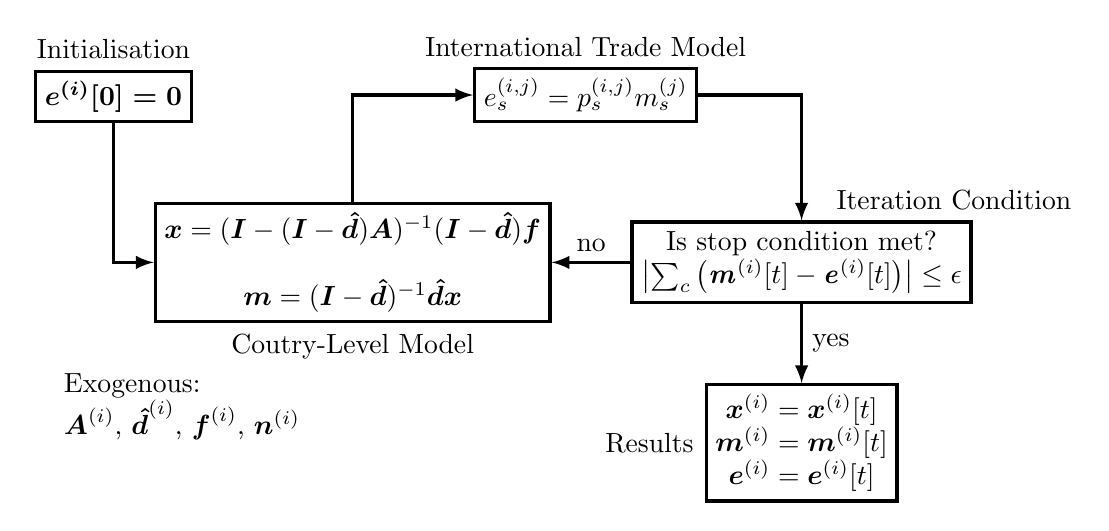
\begin{tikzpicture}[>=latex, very thick]
	\tikzstyle{all nodes}=[shape=rectangle]
	\tikzstyle{box}=[draw]
	% % Nodes
	% init
	\node[box,label=above:Initialisation](init)
	{$\boldsymbol{e^{(i)}[0] = 0}$};
	% country-level model
	\node[box, below right= and -.5cm of init, 
		  align=center, label=below:Coutry-Level Model]
	(country)
	{
		$
		\boldsymbol{x} = 
		(\boldsymbol{I} - 
		(\boldsymbol{I} - \boldsymbol{\hat{d}})
		\boldsymbol{A})^{-1} 
		(\boldsymbol{I} - \boldsymbol{\hat{d}})\boldsymbol{f}
		$ \\\\
		$
		\boldsymbol{m} = 
		(\boldsymbol{I} - 
		\boldsymbol{\hat{d}})^{-1} 
		\boldsymbol{\hat{d}}\boldsymbol{x}
		$
	};
	% international trade model
	\node[box, above right= and -1cm of country](trade)
	[label=above:International Trade Model]
	{
		$e_s^{(i,j)} = p_s^{(i,j)}m_s^{(j)}$
	};
	% iteration condition
	\node[box, right= of country, align=center](iteration)
	[label=60:Iteration Condition]
	{
		Is stop condition met?
		\\
		$
		\left| \sum_{c} \left(\textbf{\textit{m}}^{(i)}[t] -
		\textbf{\textit{e}}^{(i)}[t] \right) \right| \leq \epsilon
		$
	};
	% results
	\node[box, below=of iteration, align=center](result)
	[label=left:Results]
	{
		$\boldsymbol{x}^{(i)}=\boldsymbol{x}^{(i)}[t]$ \\
		$\boldsymbol{m}^{(i)}=\boldsymbol{m}^{(i)}[t]$ \\
		$\boldsymbol{e}^{(i)}=\boldsymbol{e}^{(i)}[t]$
	};
	% Exogenous annotation
	\node[below left=0.5cm and -2cm of country, align=left] {
	Exogenous: \\
	$\boldsymbol{A}^{(i)}$,
	$\boldsymbol{\hat{d}}^{(i)}$,
	$\boldsymbol{f}^{(i)}$,
	$\boldsymbol{n}^{(i)}$
	};
	% % Connectors
	\draw [->] (init) |- (country);
	\draw [->] (country) |- (trade);
	\draw [->] (trade) -| (iteration);
	\draw [->] (iteration) -- node[above]{no} (country);
	\draw [->] (iteration) -- node[right]{yes}(result);
\end{tikzpicture}
\caption{The model algorithm: total production, imports and exports are calculated for a given set of exogenous parameters.}\label{fig:algorithm}
\end{figure}

\section{Analysis}\label{sec:analysis}
A simple way to find the sectors most important to the global economy is to reduce by \$1 final demand for each sector in turn, measuring the effect of the other countries and sectors in the model.

Figure \ref{tbl:delta_total_output} shows the 10 largest sectors in terms of their impact on the total output, $x_s^{(i)}$,  of every other sector in every other country.
The vehicles sector in China is the most important sector by this measure, a \$1 reduction in final demand in this sector leading to a \$98.35 reduction in total output worldwide. 
Figure \ref{tbl:delta_chn_veh} shows the ten countries most affected by Chinese vehicles, as measured by the total impact on all sectors.
China itself tops this table with a \$9.55 reduction in total output due to a \$1 reduction in output from the vehicles sector.
In figure \ref{tbl:chinese_response_to_chn_vec}, the response of the Chinese economy is broken down by sector.
The electricals sector is the most strongly affected, with a \$1.62 reduction in total output. Also strongly affected are the vehicles sector itself (\$1.53), metals (\$1.44) and chemicals (\$0.95).

It might be assumed from figure \ref{tbl:chinese_response_to_chn_vec} that the electricals industry is heavily demanded by the vehicles industry, but the relevant technical coefficient is only 0.06.
It hence takes just 6\textcent{}  of electricals to make a dollar's worth of vehicles, compared to almost 12\textcent{} of metals.
Furthermore, metals is more demanded by the Chinese economy as a whole, requiring \$1.06 to make one dollar of every sector, against 77\textcent{} of electricals.


\subsection*{A random `hopper'}
Consider the problem of finding routes which products in the model might take to get from sector $r$ in country $j$ to sector $s$ in country $i$.
A random walker, or `hopper', will starting in $r$, and first decide whether to hop to another sector in $j$ or to hop abroad. The probability that the hopper hops abroad is given by the import propensity, $d_r^{(j)}$.
If hopping domestically, the hopper hops randomly to another sector, $q$, with probability proportional to the technical coefficient $a_{qr}^{(j)}$.
The coefficient $a_{rr}^{(j)}$ is set to zero to avoid paths involving sector $r$ itself.
If hopping abroad, the hopper arrives in country $k$ with a probability proportional to the import propensity $p_r^{(k,j)}$.

The hopper hops in this manner for some fixed, arbitrary number of hops.
If the hopper arrives at the destination sector, $s$ in country $i$ within this number of hops, the route taken is recorded.
When either the destination is reached or the maximum number of hops is exceeded, the hopper starts again from sector $r$ in country $j$.


\begin{figure}
	\centering
	\subfigure[response summed across all countries/sectors]
	{
		\begin{tabular}{llr}
		\toprule
		Sector & Country & $\Delta$\\
		\midrule
		      Vehicles &            China & -98.35 \\
		        Metals &            Korea & -98.27 \\
		      Vehicles &            Korea & -98.27 \\
		     Plastics &            China & -98.26 \\
		      Textiles &            China & -98.24 \\
		       Leather &            China & -98.18 \\
		     Utilities &            Korea & -98.18 \\
		          Wood &            China & -98.13 \\
		  Construction &            China & -98.11 \\
		      Vehicles &            Japan & -98.10 \\
		\bottomrule
		\end{tabular}
		\label{tbl:delta_total_output}
	}
	\subfigure[response to vehicles sector in China]
	{
		\begin{tabular}{lr}
		\toprule
		Country &     $\Delta$ \\
		\midrule
		China      & -9.56 \\
		Japan      & -8.73 \\
		USA      & -6.95 \\
		Italy      & -6.38 \\
		Germany      & -5.91 \\
		Poland      & -4.91 \\
		Czech Rep.      & -4.55 \\
		Korea      & -4.31 \\
		France      & -4.22 \\
		Brazil      & -4.18 \\
		\bottomrule
		\end{tabular}
		\label{tbl:delta_chn_veh}
	}
	\subfigure[response of Chinese sectors to vehicles sector in China]
	{
		\begin{tabular}{lr}
		\toprule
		sector & $\Delta$ \\
		\midrule
		Electricals       & -1.62 \\
		Vehicles          & -1.53 \\
		Metals            & -1.44 \\
		Chemicals         & -0.95 \\
		Machinery         & -0.54 \\
		Mining            & -0.42 \\
		Plastics          & -0.39 \\
		Utilities         & -0.35 \\
		Textiles          & -0.23 \\
		Wholesale Trade   & -0.22 \\
		\bottomrule	
		\end{tabular}
		\label{tbl:chinese_response_to_chn_vec}
	}
	\caption{Response ($\Delta$) to a \$1 reduction in final demand for the shown sector, in terms of difference in the total output, $x$, of other sectors. All tables show the largest 10 only.}
\end{figure}

%\begin{table}
%\begin{center}
%\begin{tabular}{lr}
%\toprule
%Sector &     $\sum{a}$ \\
%\midrule
%Electricals  &  0.82 \\
%Plastics     &  0.81 \\
%Fuel         &  0.80 \\
%Vehicles     &  0.80 \\
%Leather      &  0.80 \\
%Metals       &  0.79 \\
%Textiles     &  0.79 \\
%Chemicals    &  0.79 \\
%Wood         &  0.77 \\
%Construction &  0.77 \\
%\bottomrule
%\end{tabular}
%\end{center}
%\caption{The sum of all technical coefficients, $\sum_r{a_{rs}^{(CHN)}}, s=\text{electricals}$, for each sector of the Chinese economy. Only the largest 10 are shown.}\label{tbl:chn_electricals}
%\end{table}

\subsection*{A unified network approach}
The flow of goods between countries can be viewed as a weighted, directed network, where countries are nodes, and the weights of each edge represents the magnitude of the flow between them \parencite{Nystuen1961,Serrano2003,Bhattacharya2008,Baskaran2011}.
Similarly with the sector-sector flows which constitute an input-output model \parencite{Blochl2011}.
Network science has developed useful ways to analyse the sort of weighted, directed networks which the constitute the present model, but a single network representation is required which combines the international and the sub-national networks.

Recall from section \ref{sec:importratios} above, that goods arriving at the shores of an importing country are put into a warehouse along with domestically produced goods, at which point the two become indistinguishable.
Under the additional assumption that domestic sectors take from this warehouse by method of a random sample, the fraction of goods in each sample from abroad will be constant, as will the fraction of imported goods from each exporter.
These fractions will be set by the import ratios and import propensities respectively.

This additional assumption allows us to specify a complete system of flows, $y_{rs}^{(i,j)}$, from sector $r$ in country $i$ to sector $s$ in country $j$:

\begin{equation}\label{eqn:y_rsij}
y_{rs}^{(i,j)} = p_{r}^{(i,j)} d_{r}^{(j)} a_{rs}^{(j)} x_{s}^{(j)}
\end{equation}
Equation \eqref{eqn:y_rsij} can be understood as follows:
sector $s$ in country $j$ requires an amount $a_{rs}^{(j)} x_{s}^{(j)}$ of sector $r$'s good to produce its total output;
a fraction $d_{r}^{(j)}$ of this will be supplied by imports;
a fraction $p_{r}^{(i,j)}$ of these imports will come from country $i$.

Along with the sector-to-sector flows given by equation \eqref{eqn:zstar}, this allows the representation of all the flows in the present model as a single network, and standard network analysis techniques can then be used.

\section{Conclusions}\label{sec:conclusions}

\printbibliography

\end{document} 
